% THIS IS SIGPROC-SP.TEX - VERSION 3.1
% WORKS WITH V3.2SP OF ACM_PROC_ARTICLE-SP.CLS
% APRIL 2009
%
% It is an example file showing how to use the 'acm_proc_article-sp.cls' V3.2SP
% LaTeX2e document class file for Conference Proceedings submissions.
% ----------------------------------------------------------------------------------------------------------------
% This .tex file (and associated .cls V3.2SP) *DOES NOT* produce:
%       1) The Permission Statement
%       2) The Conference (location) Info information
%       3) The Copyright Line with ACM data
%       4) Page numbering
% ---------------------------------------------------------------------------------------------------------------
% It is an example which *does* use the .bib file (from which the .bbl file
% is produced).
% REMEMBER HOWEVER: After having produced the .bbl file,
% and prior to final submission,
% you need to 'insert'  your .bbl file into your source .tex file so as to provide
% ONE 'self-contained' source file.
%
% Questions regarding SIGS should be sent to
% Adrienne Griscti ---> griscti@acm.org
%
% Questions/suggestions regarding the guidelines, .tex and .cls files, etc. to
% Gerald Murray ---> murray@hq.acm.org
%
% For tracking purposes - this is V3.1SP - APRIL 2009

\documentclass{acm_proc_article-sp}

\usepackage{float}
\usepackage{graphicx}
\usepackage[utf8]{inputenc}
\usepackage{listings}

\lstset
{
    basicstyle=\ttfamily\small,
    breakatwhitespace=false,
    breaklines=true,
    frame=single,
    inputencoding=utf8,
    language=bash,
    numbers=left
}

\newcommand{\code}[1]{{\tt #1}}
\newcommand{\prog}[1]{{\tt #1}}

\newcommand{\secref}[1]{(see section \ref{#1})}
\newcommand{\figref}[1]{(see figure~\ref{#1})}

\begin{document}

\title{Datanet Assignment 1}
\subtitle{Network Tools}
%
% You need the command \numberofauthors to handle the 'placement
% and alignment' of the authors beneath the title.
%
% For aesthetic reasons, we recommend 'three authors at a time'
% i.e. three 'name/affiliation blocks' be placed beneath the title.
%
% NOTE: You are NOT restricted in how many 'rows' of
% "name/affiliations" may appear. We just ask that you restrict
% the number of 'columns' to three.
%
% Because of the available 'opening page real-estate'
% we ask you to refrain from putting more than six authors
% (two rows with three columns) beneath the article title.
% More than six makes the first-page appear very cluttered indeed.
%
% Use the \alignauthor commands to handle the names
% and affiliations for an 'aesthetic maximum' of six authors.
% Add names, affiliations, addresses for
% the seventh etc. author(s) as the argument for the
% \additionalauthors command.
% These 'additional authors' will be output/set for you
% without further effort on your part as the last section in
% the body of your article BEFORE References or any Appendices.

\numberofauthors{1} %  in this sample file, there are a *total*
% of EIGHT authors. SIX appear on the 'first-page' (for formatting
% reasons) and the remaining two appear in the \additionalauthors section.
%
\author{
% You can go ahead and credit any number of authors here,
% e.g. one 'row of three' or two rows (consisting of one row of three
% and a second row of one, two or three).
%
% The command \alignauthor (no curly braces needed) should
% precede each author name, affiliation/snail-mail address and
% e-mail address. Additionally, tag each line of
% affiliation/address with \affaddr, and tag the
% e-mail address with \email.
%
% 1st. author
\alignauthor
    Casper B. Hansen\\
    \affaddr{University of Copenhagen}\\
    \affaddr{2100 Universitetsparken 5}\\
    \affaddr{Copenhagen, Denmark}\\
    \email{fvx507@alumni.ku.dk}
}
% There's nothing stopping you putting the seventh, eighth, etc.
% author on the opening page (as the 'third row') but we ask,
% for aesthetic reasons that you place these 'additional authors'
% in the \additional authors block, viz.

\date{\today}
% Just remember to make sure that the TOTAL number of authors
% is the number that will appear on the first page PLUS the
% number that will appear in the \additionalauthors section.

\maketitle
\begin{abstract}
    An overview of the basic tools used for analyzing the behaviour of network
    systems. In a practical approach by experimenting with these tools we lead
    into a discussion of more theoretical topics in network technologies.
\end{abstract}

% A category with the (minimum) three required fields
% \category{H.4}{Information Systems Applications}{Miscellaneous}
% A category including the fourth, optional field follows...
% \category{D.2.8}{Software Engineering}{Metrics}[complexity measures, performance measures]

\terms{Experimentation, Measurement}
\keywords{Network, Tools}

\section{Introduction}
\label{sec:introduction}
I will briefly go over the system and network setup used to perform the
practical aspects discussed throughout the document. Having provided these one
can more easily reason the results of the measurements to be discussed later.

\subsection{System Setup}
\label{sec:introduction|sub:system-setup}
The system used ran in the virtual machine environment VirtualBox (4.3.8).

\begin{tabular}{ll}
    {\bf OS / Kernel}   & Arch Linux / 3.14.1-1-ARCH \\
    {\bf User / Host}   & casperbhansen / arch \\
\end{tabular}

All programs used were acquired through {\it pacman}, which is the
standard package manager for Arch Linux.

\subsection{Network Setup}
\label{sec:introduction|sub:network-setup}
The network was driven via the host computer, as a bridged connection,
through the host system running Mac OS 10.9.2.

\begin{tabular}{ll}
    {\bf Speed (Up/Down)}   & 1 Mbit / 10 Mbit \\
    {\bf Connection}        & Wireless \\
\end{tabular}

Because the connection is bridged, the test results should suffer little
impact. However, since the connection is wireless some induced latency is to
be expected.

\section{Latency and Bandwidth}
\label{sec:latency-and-bandwidth}
By experimentation with tools like \prog{ping}, \prog{traceroute} and
\prog{wget} on the chosen target network hosts and a discussion of the
results we can attempt to draw a few conclusions.

\subsection{Chosen Targets}
\label{sec:latency-and-bandwidth|sub:chosen-targets}
For convenience, I have listed the target network hosts that will be tested
against. Each target is assigned a shorthand label for easy reference.
\begin{center}
    \begin{tabular}{|c|c|c|}
        \hline
        {\bf Label}     & {\bf Location}    & {\bf URL} \\ \hline
        AU  & Australia & {\tt http://ftp.au.debian.org/debian/} \\ \hline
        DK  & Denmark   & {\tt http://ftp.dk.debian.org/debian/} \\ \hline
        JP  & Japan     & {\tt http://ftp.jp.debian.org/debian/} \\ \hline
        UK  & England   & {\tt http://ftp.uk.debian.org/debian/} \\ \hline
        US  & America   & {\tt http://ftp.us.debian.org/debian/} \\ \hline
    \end{tabular}
\end{center}
The targets were chosen with the intend of producing a variety of results. The
tests were conducted in Denmark, making the Danish mirror the closest. England
comes in second as it is relatively close to Denmark. For the remainder of the
targets many factors can influence which is the fastest and slowest, so I
won't be making any guesses --- these were selected for exactly this reason.

\subsection{Ping}
\label{sec:latency-and-bandwidth|sub:ping}
The \prog{ping} program sends out an ICMP\footnote{ICMP --- Acronym for {\it
Internet Control Message Protocol}.} \code{ECHO\_REQUEST} datagram, consisting
of an IP-address  ICMP header and a timeval structure[\prog{ping} manual
page]. An \code{ECHO\_REQUEST} can be thought of as the {\it ``ping''} itself,
which basically asks the target network host to send back an ICMP
\code{ECHO\_REPLY}, also known as a {\it ``pong''}.

\begin{figure}[H]
    \center
    \begin{tabular}{|c|c|c|c|}
        \hline
        {\bf Target} & {\bf Minimum} & {\bf Average} & {\bf Maximum} \\ \hline
        DK & 31.649 ms  & 33.972 ms  & 36.685 ms \\ \hline
        UK & 42.757 ms  & 52.393 ms  & 71.944 ms \\ \hline
        US & 120.464 ms & 193.454 ms & 243.455 ms \\ \hline
        JP & 350.175 ms & 391.000 ms & 434.614 ms \\ \hline
        AU & 424.835 ms & 461.892 ms & 502.756 ms \\ \hline
    \end{tabular}
    \caption{Ping summary of results}
    \label{table:ping}
\end{figure}

The above table shows the set of results for each target, sorted by average
response time.

As to be expected, the fastest response time was the destination closest to
the source (DK).

\subsection{Trace Route}
\label{sec:latency-and-bandwidth|sub:traceroute}
Examining the \prog{traceroute} outputs \secref{sec:appendix|sub:traceroute}
for the chosen targets \secref{sec:latency-and-bandwidth|sub:chosen-targets}
we look at the routes taken to reach the destination. We begin by highlighting
the most interesting case. Before performing the test, I would have guessed
that the route taken to reach Australia would have been through Asia --- that
is, I had expected it to choose a guided media route over an unguided.

\begin{figure}[H]
    \center
    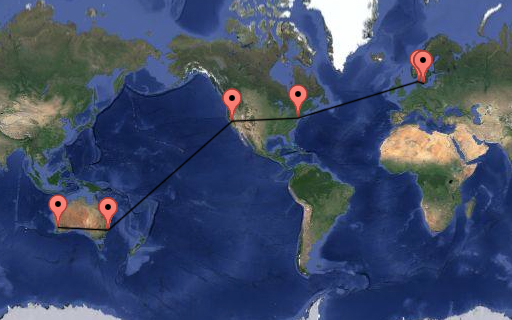
\includegraphics[scale=0.47]{figures/traceroute_au.jpg}
    \caption{Visual representation of a traceroute from Denmark to Australia}
    \label{fig:traceroute-australia}
\end{figure}

However, by the route taken, as represented in the above figure, we see that
two satellite relay routes are taken. This was unexpected as the unguided
media of satellite links produce a substantially high latency, mostly due to
the signal propagation delay, suggested\cite[p. 21]{KR} to be around 280 ms.

Before leaving Denmark, the route taken must at least pass an ISP central, as
such lines 2--8 are found in all of the \prog{traceroute} outputs. Lines 4--7
constitute the local ISP, while line 8 constitutes the global ISP.

\subsection{Wget}
\label{sec:latency-and-bandwidth|sub:wget}
Using a tool such as \prog{wget} we can download files from the internet. For
purposes of testing stability of a network connection over time, I've chosen a
rather large file to download; the latest (at the time of writing)
distribution of Arch Linux.

The file to be downloaded is 565.182.464 bytes in size $L$. With a downstream
bandwidth $R$ of 10 Mbit/s at our disposal, we can calculate the expected time
it takes to download the file, given that the circumstances are optimal.

\begin{align}
    \frac{L}{R}
    &= \frac{565.182.464 \text{ bytes} \cdot 8 \text{ bits}}
            {10 \text{ Mbit/s} \cdot 1024^2}
     = 431,2 \text{ seconds}
\end{align}

As evident from the output of \prog{wget} \figref{fig:wget-output}, the
transmission delay, as calculated above, is relatively close to the time it
took to download the file, which took 9 minutes and 20 seconds. Or, 560
seconds, to be more precise, making the transmission delay the dominant term
of the total delay. The remainder of the total delay constitutes processing,
queuing and propagation delay. This example was selected to exemplify the
transmission delay. Had we chosen a small target file that required a one or
more satellite links, the propagation delay would likely become the dominant
term, as the signal would take longer to reach, or propagate, to us.

\begin{figure}[H]
    \lstinputlisting{logs/wget.out}
    \caption{Output log from \prog{wget}}
    \label{fig:wget-output}
\end{figure}

\section{HTTP Protocol}
\label{sec:http-protocol}
Using the tool \prog{Wireshark} we can examine the data transmission
correspondence between a client and a server. With the intent of gaining an
understanding of how a network application can improve its performance by
employing the concept of caching.

\subsection{Hypothesis}
\label{sec:http-protocol|sub:hypothesis}
Recently requested data is likely to be requested more than once when browsing
the web. Therefore any intermediary channels (e.g. proxy servers) should cache
these data for future requests, including the local client. This alleviates
unnecessary network traffic. By this I reason that the second trace should be
far smaller than the first.

\subsection{Experiment}
\label{sec:http-protocol|sub:experiment}
A web browser (in this case, we will use Google's Chromium) is cleared of all
of its cached data. The URL\\{\tt http://www.diku.dk/} is then requested. Upon
having received the response the browser is closed and reopened, and the same
URL is revisited. The traces are then compared.

\subsection{Results}
\label{sec:http-protocol|sub:results}
The first ---uncached--- trace produces a massive amount of data
transmissions; 1987 recorded transmissions to be exact. The following
---cached--- trace produces a mere 106 \secref{sec:appendix|sub:trace-cached}
recorded transmissions. These results are in agreement with the posed
hypothesis.

% Single appendix
%
% \section*{APPENDIX}
% \setcounter{section}{1}
% ...

% Multiple appendices
%
% \appendix
% \section*{APPENDIX}
% \section{First}
% \section{Second}

% \ack{}

%
% The following two commands are all you need in the
% initial runs of your .tex file to
% produce the bibliography for the citations in your paper.
\bibliographystyle{abbrv}
\bibliography{sigproc}  % sigproc.bib is the name of the Bibliography in this case
\begin{thebibliography}{9}
    
    \bibitem{KR}
        James F. Kurose, Keith W. Ross,\\
        \emph{Computer Networking, A Top-Down Approach},\\
        Pearson Education, Sixth Edition, 2013
    
\end{thebibliography}

% You must have a proper ".bib" file
%  and remember to run:
% latex bibtex latex latex
% to resolve all references
%
% ACM needs 'a single self-contained file'!
%
% APPENDICES are optional
\balancecolumns
\onecolumn
\appendix

% Appendix A
\section{OUTPUT LOGS}

\subsection{Trace route}
\label{sec:appendix|sub:traceroute}
\begin{figure}[H]
    \lstinputlisting{logs/traceroute_au.out}
    \caption{Traceroute results of {\tt ftp.au.debian.org}}
    \label{fig:traceroute-au}
\end{figure}

\begin{figure}[H]
    \lstinputlisting{logs/traceroute_us.out}
    \caption{Traceroute results of {\tt ftp.us.debian.org}}
    \label{fig:traceroute-us}
\end{figure}

\begin{figure}[H]
    \lstinputlisting{logs/traceroute_dk.out}
    \caption{Traceroute results of {\tt ftp.dk.debian.org}}
    \label{fig:traceroute-dk}
\end{figure}

\begin{figure}[H]
    \lstinputlisting{logs/traceroute_jp.out}
    \caption{Traceroute results of {\tt ftp.jp.debian.org}}
    \label{fig:traceroute-jp}
\end{figure}

\begin{figure}[H]
    \lstinputlisting{logs/traceroute_uk.out}
    \caption{Traceroute results of {\tt ftp.uk.debian.org}}
    \label{fig:traceroute-uk}
\end{figure}

\subsection{Cached Wireshark Trace}
\label{sec:appendix|sub:trace-cached}
{\ }
\lstinputlisting{logs/cached_request.log}

% \section{Appendix B}

\end{document}
